% Options for packages loaded elsewhere
\PassOptionsToPackage{unicode}{hyperref}
\PassOptionsToPackage{hyphens}{url}
%
\documentclass[
]{article}
\usepackage{amsmath,amssymb}
\usepackage{lmodern}
\usepackage{iftex}
\ifPDFTeX
  \usepackage[T1]{fontenc}
  \usepackage[utf8]{inputenc}
  \usepackage{textcomp} % provide euro and other symbols
\else % if luatex or xetex
  \usepackage{unicode-math}
  \defaultfontfeatures{Scale=MatchLowercase}
  \defaultfontfeatures[\rmfamily]{Ligatures=TeX,Scale=1}
\fi
% Use upquote if available, for straight quotes in verbatim environments
\IfFileExists{upquote.sty}{\usepackage{upquote}}{}
\IfFileExists{microtype.sty}{% use microtype if available
  \usepackage[]{microtype}
  \UseMicrotypeSet[protrusion]{basicmath} % disable protrusion for tt fonts
}{}
\makeatletter
\@ifundefined{KOMAClassName}{% if non-KOMA class
  \IfFileExists{parskip.sty}{%
    \usepackage{parskip}
  }{% else
    \setlength{\parindent}{0pt}
    \setlength{\parskip}{6pt plus 2pt minus 1pt}}
}{% if KOMA class
  \KOMAoptions{parskip=half}}
\makeatother
\usepackage{xcolor}
\usepackage[margin=1in]{geometry}
\usepackage{color}
\usepackage{fancyvrb}
\newcommand{\VerbBar}{|}
\newcommand{\VERB}{\Verb[commandchars=\\\{\}]}
\DefineVerbatimEnvironment{Highlighting}{Verbatim}{commandchars=\\\{\}}
% Add ',fontsize=\small' for more characters per line
\usepackage{framed}
\definecolor{shadecolor}{RGB}{248,248,248}
\newenvironment{Shaded}{\begin{snugshade}}{\end{snugshade}}
\newcommand{\AlertTok}[1]{\textcolor[rgb]{0.94,0.16,0.16}{#1}}
\newcommand{\AnnotationTok}[1]{\textcolor[rgb]{0.56,0.35,0.01}{\textbf{\textit{#1}}}}
\newcommand{\AttributeTok}[1]{\textcolor[rgb]{0.77,0.63,0.00}{#1}}
\newcommand{\BaseNTok}[1]{\textcolor[rgb]{0.00,0.00,0.81}{#1}}
\newcommand{\BuiltInTok}[1]{#1}
\newcommand{\CharTok}[1]{\textcolor[rgb]{0.31,0.60,0.02}{#1}}
\newcommand{\CommentTok}[1]{\textcolor[rgb]{0.56,0.35,0.01}{\textit{#1}}}
\newcommand{\CommentVarTok}[1]{\textcolor[rgb]{0.56,0.35,0.01}{\textbf{\textit{#1}}}}
\newcommand{\ConstantTok}[1]{\textcolor[rgb]{0.00,0.00,0.00}{#1}}
\newcommand{\ControlFlowTok}[1]{\textcolor[rgb]{0.13,0.29,0.53}{\textbf{#1}}}
\newcommand{\DataTypeTok}[1]{\textcolor[rgb]{0.13,0.29,0.53}{#1}}
\newcommand{\DecValTok}[1]{\textcolor[rgb]{0.00,0.00,0.81}{#1}}
\newcommand{\DocumentationTok}[1]{\textcolor[rgb]{0.56,0.35,0.01}{\textbf{\textit{#1}}}}
\newcommand{\ErrorTok}[1]{\textcolor[rgb]{0.64,0.00,0.00}{\textbf{#1}}}
\newcommand{\ExtensionTok}[1]{#1}
\newcommand{\FloatTok}[1]{\textcolor[rgb]{0.00,0.00,0.81}{#1}}
\newcommand{\FunctionTok}[1]{\textcolor[rgb]{0.00,0.00,0.00}{#1}}
\newcommand{\ImportTok}[1]{#1}
\newcommand{\InformationTok}[1]{\textcolor[rgb]{0.56,0.35,0.01}{\textbf{\textit{#1}}}}
\newcommand{\KeywordTok}[1]{\textcolor[rgb]{0.13,0.29,0.53}{\textbf{#1}}}
\newcommand{\NormalTok}[1]{#1}
\newcommand{\OperatorTok}[1]{\textcolor[rgb]{0.81,0.36,0.00}{\textbf{#1}}}
\newcommand{\OtherTok}[1]{\textcolor[rgb]{0.56,0.35,0.01}{#1}}
\newcommand{\PreprocessorTok}[1]{\textcolor[rgb]{0.56,0.35,0.01}{\textit{#1}}}
\newcommand{\RegionMarkerTok}[1]{#1}
\newcommand{\SpecialCharTok}[1]{\textcolor[rgb]{0.00,0.00,0.00}{#1}}
\newcommand{\SpecialStringTok}[1]{\textcolor[rgb]{0.31,0.60,0.02}{#1}}
\newcommand{\StringTok}[1]{\textcolor[rgb]{0.31,0.60,0.02}{#1}}
\newcommand{\VariableTok}[1]{\textcolor[rgb]{0.00,0.00,0.00}{#1}}
\newcommand{\VerbatimStringTok}[1]{\textcolor[rgb]{0.31,0.60,0.02}{#1}}
\newcommand{\WarningTok}[1]{\textcolor[rgb]{0.56,0.35,0.01}{\textbf{\textit{#1}}}}
\usepackage{graphicx}
\makeatletter
\def\maxwidth{\ifdim\Gin@nat@width>\linewidth\linewidth\else\Gin@nat@width\fi}
\def\maxheight{\ifdim\Gin@nat@height>\textheight\textheight\else\Gin@nat@height\fi}
\makeatother
% Scale images if necessary, so that they will not overflow the page
% margins by default, and it is still possible to overwrite the defaults
% using explicit options in \includegraphics[width, height, ...]{}
\setkeys{Gin}{width=\maxwidth,height=\maxheight,keepaspectratio}
% Set default figure placement to htbp
\makeatletter
\def\fps@figure{htbp}
\makeatother
\setlength{\emergencystretch}{3em} % prevent overfull lines
\providecommand{\tightlist}{%
  \setlength{\itemsep}{0pt}\setlength{\parskip}{0pt}}
\setcounter{secnumdepth}{-\maxdimen} % remove section numbering
\ifLuaTeX
  \usepackage{selnolig}  % disable illegal ligatures
\fi
\IfFileExists{bookmark.sty}{\usepackage{bookmark}}{\usepackage{hyperref}}
\IfFileExists{xurl.sty}{\usepackage{xurl}}{} % add URL line breaks if available
\urlstyle{same} % disable monospaced font for URLs
\hypersetup{
  pdftitle={Práctica dirigida 5},
  hidelinks,
  pdfcreator={LaTeX via pandoc}}

\title{Práctica dirigida 5}
\author{}
\date{\vspace{-2.5em}}

\begin{document}
\maketitle

{
\setcounter{tocdepth}{1}
\tableofcontents
}
\hypertarget{revisemos-lo-avanzado-sobre-estaduxedstica-inferencial}{%
\section{\texorpdfstring{\textbf{Revisemos lo avanzado sobre estadística
inferencial}}{Revisemos lo avanzado sobre estadística inferencial}}\label{revisemos-lo-avanzado-sobre-estaduxedstica-inferencial}}

En esta sesión repasaremos lo revisado hasta el momento sobre
estadística inferencial: intervalos de confianza, prueba T y revisamos
comparación de proporciones.

La base a usar en esta sesión (``data-paises.xlsx'') proviene de la
unión de tres bases de datos distintas, estas son ``Human Development
Index'' elaborada por UNDP
(\href{https://hdr.undp.org/data-center/documentation-and-downloads}{https://hdr.undp.org/data-center/documentation-and-downloads)},);
``Index of Economic Freedom'' realizada por Heritage Foundation
(\href{https://indexdotnet.azurewebsites.net/index/explore}{https://indexdotnet.azurewebsites.net/index/explore)})
y ``Fragile State Index'' elaborada por The Fund For Peace
(\href{https://fragilestatesindex.org/global-data/}{https://fragilestatesindex.org/global-data/).}.)
Asimismo, los datos con los que trabajaremos corresponden a información
del 2021 y la unidad de análisis son países.

Sobre las bases de estudio:

\begin{itemize}
\item
  El Human Development Index mide el índice de desarrollo humano a
  través de 3 aspectos: esperanza de vida, educación e ingresos per
  cápita. Su escala es de 0 a 1.
\item
  El Index of Economic Freedom mide el grado de libertad económica
  mediante 12 indicadores agrupados en 4 categorías: Estado de Derecho,
  tamaño de Gobierno, eficiencia regulatoria y apertura de mercados.
\item
  El Fragile State Index mide la fragilidad de un Estado a través de 12
  indicadores agrupados en 4 categorías: cohesión, economía, política y
  social. Su escala es de 0 a 120.
\end{itemize}

\begin{Shaded}
\begin{Highlighting}[]
\CommentTok{\#Llamemos al paquete}
\FunctionTok{library}\NormalTok{(rio)}
\NormalTok{data}\OtherTok{=}\FunctionTok{import}\NormalTok{(}\StringTok{"data{-}paises.xlsx"}\NormalTok{)}
\CommentTok{\#Llamemos a nuestra base de datos}
\end{Highlighting}
\end{Shaded}

\hypertarget{prueba-t}{%
\section{\texorpdfstring{\textbf{Prueba T}}{Prueba T}}\label{prueba-t}}

Recuerda que hay condiciones para poder realizar la prueba T:

\begin{itemize}
\item
  Independencia: Las muestras deben ser independientes. El muestreo debe
  ser aleatorio.
\item
  Igualdad de varianza: La varianza de ambas poblaciones comparadas debe
  ser igual. \emph{(Prueba Levene)}
\item
  La variable numérica se distribuye de manera normal.
\end{itemize}

\hypertarget{pasos-para-realizar-la-prueba-t}{%
\subsubsection{\texorpdfstring{\textbf{Pasos para realizar la Prueba
T}}{Pasos para realizar la Prueba T}}\label{pasos-para-realizar-la-prueba-t}}

\begin{enumerate}
\def\labelenumi{\arabic{enumi}.}
\tightlist
\item
  Establecer hipótesis
\item
  Calcular el estadístico (parámetro estimado) que se va a emplear
\item
  Determinar el nivel de significancia α (alpha)
\item
  Calcular el p-value y realizar la prueba t.test
\item
  Interpretar
\end{enumerate}

Apliquemos lo revisado\ldots{}

Primero, exploraremos un poco las variables de interés:

V27: Índice de desarrollo humano V1: Índice de libertad económica

Ambas variables son numéricas, inicialmente. Sin embargo para la prueba
T es necesario contar con una variable numérica y otra categórica. Es
así que crearemos 2 grupos según la variable V1 (Que puede ir del 0 al
100).

Siendo los niveles: ``Bajo'' = si es menor o igual a 50, y,
``Medio/Alto'' = si es mayor a 50

¿Cómo lo haremos? Con case when!

\begin{Shaded}
\begin{Highlighting}[]
\FunctionTok{library}\NormalTok{(tidyverse)}
\FunctionTok{summary}\NormalTok{(data}\SpecialCharTok{$}\NormalTok{V1)}
\end{Highlighting}
\end{Shaded}

\begin{verbatim}
##    Min. 1st Qu.  Median    Mean 3rd Qu.    Max. 
##   24.70   55.67   62.00   61.95   69.35   89.70
\end{verbatim}

Si revisamos el summary

\begin{Shaded}
\begin{Highlighting}[]
\NormalTok{data }\OtherTok{=}\NormalTok{ data }\SpecialCharTok{\%\textgreater{}\%}
  \FunctionTok{mutate}\NormalTok{(}
   \AttributeTok{grupo\_ILE=} \FunctionTok{case\_when}\NormalTok{(V1}\SpecialCharTok{\textless{}=}\DecValTok{50} \SpecialCharTok{\textasciitilde{}} \StringTok{"1. Bajo"}\NormalTok{, V1}\SpecialCharTok{\textgreater{}}\DecValTok{50} \SpecialCharTok{\textasciitilde{}} \StringTok{"2.Medio/Alto"}\NormalTok{))}
\end{Highlighting}
\end{Shaded}

La variable ``V27'' ya es númerica por lo que no añadimos cambios.

Ahora, analizaremos la varianza en los grupos, para ello usaremos la
prueba Levene:

H0: La varianza del Índice de Libertad Económica (en grupos) es igual a
la varianza del Índice de Desarrollo Humano. H1: La varianza del Índice
de Libertad Económica (en grupos) NO es igual a la varianza del Índice
de Desarrollo Humano.

\begin{Shaded}
\begin{Highlighting}[]
\FunctionTok{library}\NormalTok{(DescTools)}
\FunctionTok{LeveneTest}\NormalTok{(data}\SpecialCharTok{$}\NormalTok{V27, data}\SpecialCharTok{$}\NormalTok{grupo\_ILE)}
\end{Highlighting}
\end{Shaded}

\begin{verbatim}
## Levene's Test for Homogeneity of Variance (center = median)
##        Df F value Pr(>F)
## group   1  0.4909 0.4845
##       166
\end{verbatim}

Como el p valor es mayor a 0.05 podemos afirmar que las varianzas son
iguales, por lo que podemos realizar la Prueba T.

\hypertarget{realizamos-la-prueba-t}{%
\subsubsection{\texorpdfstring{\textbf{Realizamos la Prueba
T}}{Realizamos la Prueba T}}\label{realizamos-la-prueba-t}}

\hypertarget{primer-paso-establecer-la-hipuxf3tesis.}{%
\paragraph{\texorpdfstring{\textbf{Primer paso: Establecer la
hipótesis.}}{Primer paso: Establecer la hipótesis.}}\label{primer-paso-establecer-la-hipuxf3tesis.}}

La hipotesis de la prueba T queda establecida de la siguiente forma:

\begin{itemize}
\item
  H0: No hay diferencia de promedio en los niveles del Índice de
  desarrollo humano entre aquellos países que tienen un índice libertad
  económica ``Bajo'' y los que tienen un índice libertad económica
  ``Medio/Alto'' \textbf{(no diferencia de medias)}
\item
  H1: Si hay diferencia de promedio en los niveles del Índice de
  desarrollo humano entre aquellos países que tienen un índice libertad
  económica ``Bajo'' y los que tienen un índice libertad económica
  ``Medio/Alto'' \textbf{(sí diferencia de medias)}
\end{itemize}

Ambas hipótesis son acerca de los parámetros de la población.

\hypertarget{segundo-paso-calcular-el-estaduxedstico-a-emplear}{%
\paragraph{\texorpdfstring{\textbf{Segundo paso: Calcular el estadístico
a
emplear}}{Segundo paso: Calcular el estadístico a emplear}}\label{segundo-paso-calcular-el-estaduxedstico-a-emplear}}

Para verificar la diferencia de medias se calcula el estadístico T, y
uno de los primeros pasos es calcular las diferencias entre las medias
muestrales, ya que es lo quiero extrapolar y por tanto saber si existe o
no una diferencia significativa entre las medias poblacionales de ambos
grupos:

\begin{Shaded}
\begin{Highlighting}[]
\FunctionTok{library}\NormalTok{(lsr)}
\NormalTok{tabla}\OtherTok{=}\NormalTok{data}\SpecialCharTok{\%\textgreater{}\%}
  \FunctionTok{group\_by}\NormalTok{(grupo\_ILE) }\SpecialCharTok{\%\textgreater{}\%}
\FunctionTok{summarise}\NormalTok{(}\AttributeTok{Desviacion =} \FunctionTok{sd}\NormalTok{(V27, }\AttributeTok{na.rm=}\NormalTok{T),}
          \AttributeTok{Media =} \FunctionTok{mean}\NormalTok{(V27, }\AttributeTok{na.rm=}\NormalTok{T),}
            \AttributeTok{min =} \FunctionTok{ciMean}\NormalTok{(V27,}\AttributeTok{conf =} \FloatTok{0.95}\NormalTok{, }\AttributeTok{na.rm=}\NormalTok{T)[}\DecValTok{1}\NormalTok{],}
            \AttributeTok{max =} \FunctionTok{ciMean}\NormalTok{(V27,}\AttributeTok{conf =} \FloatTok{0.95}\NormalTok{, }\AttributeTok{na.rm=}\NormalTok{T)[}\DecValTok{2}\NormalTok{],}
          \AttributeTok{n=}\FunctionTok{length}\NormalTok{(V27))}
            
\NormalTok{tabla}
\end{Highlighting}
\end{Shaded}

\begin{verbatim}
##   Desviacion     Media       min      max   n
## 1  0.1528323 0.7222738 0.6989947 0.745553 168
\end{verbatim}

\hypertarget{tercer-paso-determinar-el-nivel-de-significancia}{%
\paragraph{\texorpdfstring{\textbf{Tercer paso: Determinar el nivel de
significancia}}{Tercer paso: Determinar el nivel de significancia}}\label{tercer-paso-determinar-el-nivel-de-significancia}}

De manera convencional establecemos la siguiente regla para nuestra
prueba T:

\begin{itemize}
\item
  p-value\textbackslash\textless=0.05 Rechazo la H0 y acepto H1
\item
  p-value\textbackslash\textgreater0.05 No rechazo la H0
\end{itemize}

\hypertarget{cuarto-paso-calcular-el-p-value-y-realizar-la-prueba-t.test}{%
\paragraph{\texorpdfstring{\textbf{Cuarto paso: Calcular el p-value y
realizar la prueba
t.test}}{Cuarto paso: Calcular el p-value y realizar la prueba t.test}}\label{cuarto-paso-calcular-el-p-value-y-realizar-la-prueba-t.test}}

Recuerda que el p-value mide la probabilidad de observar en una muestra
una diferencia de medias como la observada, si la diferencia de medias
poblacional fuera cero.

\begin{Shaded}
\begin{Highlighting}[]
\FunctionTok{t.test}\NormalTok{(V27 }\SpecialCharTok{\textasciitilde{}}\NormalTok{ grupo\_ILE, }\AttributeTok{data =}\NormalTok{ data,}
  \AttributeTok{alternative =} \StringTok{"two.sided"}\NormalTok{, }
  \AttributeTok{conf.level  =} \FloatTok{0.95} \CommentTok{\#nivel de confianza (95\%)}
\NormalTok{)}
\end{Highlighting}
\end{Shaded}

\begin{verbatim}
## 
##  Welch Two Sample t-test
## 
## data:  V27 by grupo_ILE
## t = -3.6649, df = 19.566, p-value = 0.001583
## alternative hypothesis: true difference in means between group 1. Bajo and group 2.Medio/Alto is not equal to 0
## 95 percent confidence interval:
##  -0.19840150 -0.05434192
## sample estimates:
##      mean in group 1. Bajo mean in group 2.Medio/Alto 
##                  0.6079375                  0.7343092
\end{verbatim}

\hypertarget{quinto-paso-interpretar}{%
\paragraph{\texorpdfstring{\textbf{Quinto paso:
Interpretar}}{Quinto paso: Interpretar}}\label{quinto-paso-interpretar}}

\textbf{¿Cómo interpreto?}

Recordando nuestras hipotesis:

\begin{itemize}
\item
  H0: No hay diferencia de promedio en los niveles de IDH entre aquellos
  países que tienen un índice de libertad económica ``Bajo'' y los que
  tienen un índice de libertad económica ``Medio / Alto''
\item
  H1: Sí hay diferencia de promedio en los niveles de IDH entre aquellos
  países que tienen un índice de libertad económica ``Bajo'' y los que
  tienen un índice de libertad económica ``Medio / Alto''
\end{itemize}

Asimismo, en el paso 4, determinamos el nivel de significancia de la
siguiente manera:

\begin{itemize}
\item
  Si el p-value del t test es \textless=0.05 Rechazo la H0 y se afirma
  H1.
\item
  Si el p-value del t test es \textgreater0.05 No rechazo la H0
\end{itemize}

Entonces, vemos que el p-value es menor a 0.05, entonces rechazo la H0,
por tanto, existe una diferencia estadísticamente significativa entre
las medias del IDH entre los países que tienen un Índice de libertad
económica ``Bajo'' y los países que tiene un Índice de libertad
económica ``Medio /Alto''.

\hypertarget{paso-final-graficar}{%
\paragraph{\texorpdfstring{\textbf{Paso FINAL:
Graficar}}{Paso FINAL: Graficar}}\label{paso-final-graficar}}

Otro método para evaluar la comparación entre grupos es realizar un
gráfico de medias con intervalos de confianza de cada grupo.

Para calcular la diferencia de medias

\begin{Shaded}
\begin{Highlighting}[]
\FunctionTok{library}\NormalTok{(Rmisc)}
\NormalTok{ic\_grupo }\OtherTok{=} \FunctionTok{group.CI}\NormalTok{(V27}\SpecialCharTok{\textasciitilde{}}\NormalTok{grupo\_ILE,data)}
\NormalTok{ic\_grupo}
\end{Highlighting}
\end{Shaded}

\begin{verbatim}
##      grupo_ILE V27.upper  V27.mean V27.lower
## 1      1. Bajo 0.6766740 0.6079375 0.5392010
## 2 2.Medio/Alto 0.7584273 0.7343092 0.7101911
\end{verbatim}

\textbf{Barras de Error}

\begin{Shaded}
\begin{Highlighting}[]
\FunctionTok{library}\NormalTok{(ggplot2)}

\FunctionTok{ggplot}\NormalTok{(ic\_grupo, }\FunctionTok{aes}\NormalTok{(}\AttributeTok{x=}\NormalTok{ grupo\_ILE, }\AttributeTok{y =}\NormalTok{V27.mean)) }\SpecialCharTok{+}
  \FunctionTok{geom\_errorbar}\NormalTok{(}\FunctionTok{aes}\NormalTok{(}\AttributeTok{ymin=}\NormalTok{V27.lower, }\AttributeTok{ymax=}\NormalTok{V27.upper), }\AttributeTok{width =} \FloatTok{0.2}\NormalTok{)}\SpecialCharTok{+}
   \FunctionTok{geom\_text}\NormalTok{(}\FunctionTok{aes}\NormalTok{(}\AttributeTok{label=}\FunctionTok{paste}\NormalTok{(}\FunctionTok{round}\NormalTok{(V27.mean,}\DecValTok{1}\NormalTok{))), }\AttributeTok{size=}\DecValTok{3}\NormalTok{)}\SpecialCharTok{+}
  \FunctionTok{xlab}\NormalTok{(}\StringTok{"Índice de Libertad Económica"}\NormalTok{) }\SpecialCharTok{+} \FunctionTok{ylab}\NormalTok{(}\StringTok{"Índice de Desarrollo Humano"}\NormalTok{)}
\end{Highlighting}
\end{Shaded}

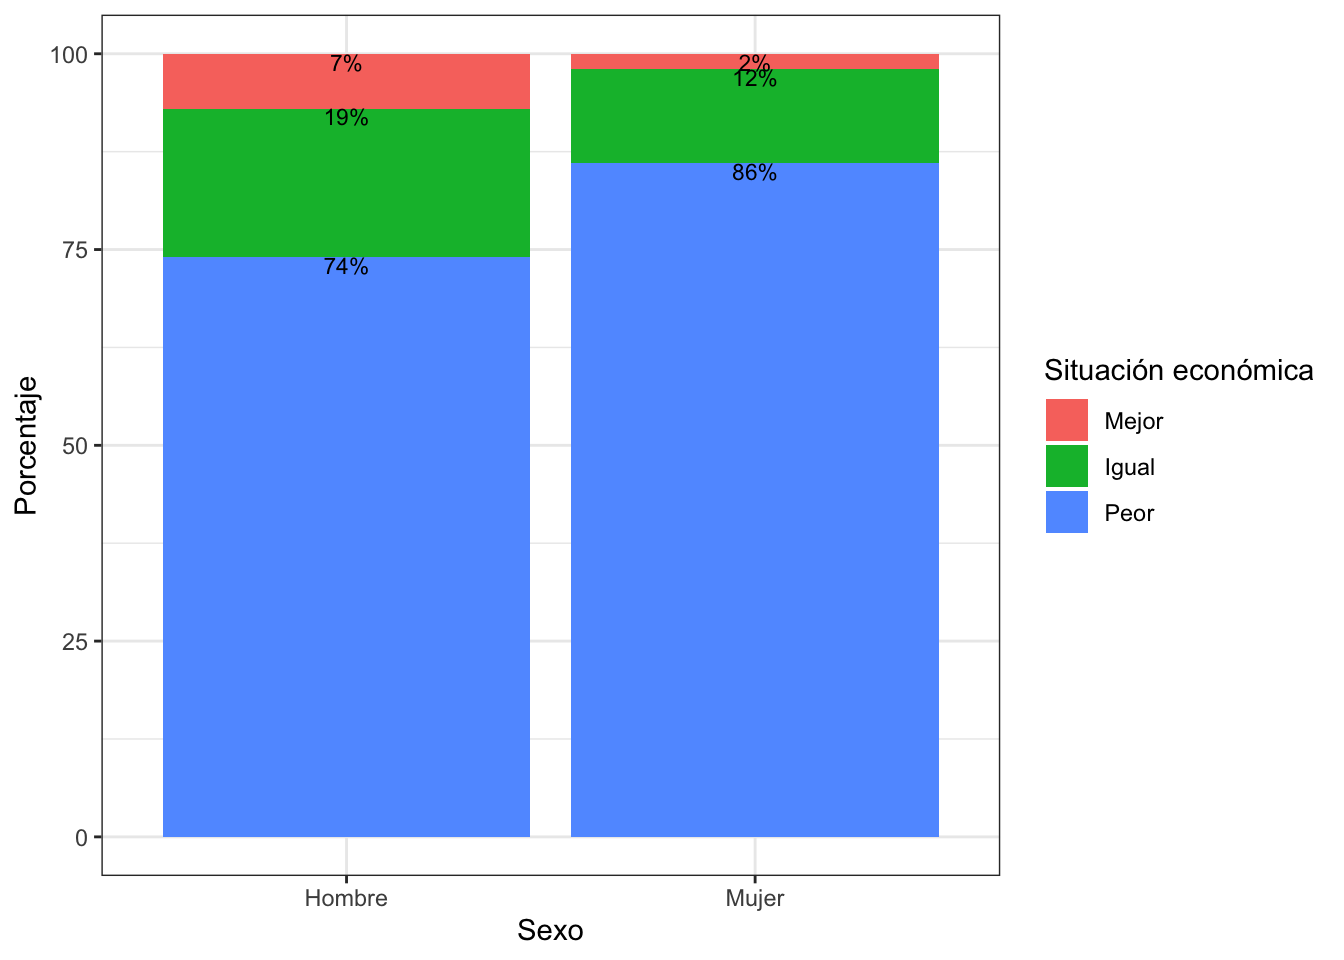
\includegraphics{pd5_files/figure-latex/unnamed-chunk-9-1.pdf}

\textbf{Interpretación}: Tal como se observa ambos intervalos de
confianza no se traslapan, por lo que se puede concluir gráficamente que
existe una diferencia estadísticamente significativa entre los grupos.
El grupo que tiene un índice de libertad económica ``Medio/Alto'' tiene
mayor IDH que el grupo que tiene un indíce de libertad económica
``Bajo'' con un 95\% de confianza.

\hypertarget{comparaciuxf3n-de-proporciones}{%
\section{\texorpdfstring{\textbf{Comparación de
proporciones}}{Comparación de proporciones}}\label{comparaciuxf3n-de-proporciones}}

Para este ejercicio trabajaremos con dos variables:

\begin{itemize}
\item
  \emph{V20: Legitimidad del Estado}
\item
  \emph{V21: Servicios públicos}
\end{itemize}

Revisemos a nuestras variables

Variable V20:

\begin{Shaded}
\begin{Highlighting}[]
\FunctionTok{class}\NormalTok{(data}\SpecialCharTok{$}\NormalTok{V20) }\CommentTok{\#Revisamos como está catalogada nuestra variable}
\end{Highlighting}
\end{Shaded}

\begin{verbatim}
## [1] "numeric"
\end{verbatim}

\begin{Shaded}
\begin{Highlighting}[]
\FunctionTok{summary}\NormalTok{(data}\SpecialCharTok{$}\NormalTok{V20) }
\end{Highlighting}
\end{Shaded}

\begin{verbatim}
##    Min. 1st Qu.  Median    Mean 3rd Qu.    Max. 
##   0.500   3.600   6.250   5.593   7.725  10.000
\end{verbatim}

Recordemos que para comparar proporciones necesitamos que nuestra
variable sea categórica. La recodificaremos para que tengamos dos
grupos: Baja/Media (de 7.73 a menos) y Alta (más de 7.73).

\begin{Shaded}
\begin{Highlighting}[]
\FunctionTok{library}\NormalTok{(tidyverse)}\CommentTok{\#Llamemos al paquete}
\NormalTok{data }\OtherTok{=}\NormalTok{ data }\SpecialCharTok{\%\textgreater{}\%}
  \FunctionTok{mutate}\NormalTok{(}\AttributeTok{V20\_2 =} \FunctionTok{case\_when}\NormalTok{(V20 }\SpecialCharTok{\textless{}=} \FloatTok{7.73} \SpecialCharTok{\textasciitilde{}} \StringTok{"Baja/Media"}\NormalTok{,}
                          \ConstantTok{TRUE} \SpecialCharTok{\textasciitilde{}} \StringTok{"Alta"}\NormalTok{))}
\end{Highlighting}
\end{Shaded}

Realizamos el mismo ejercicio con nuestra variable V21:

\begin{Shaded}
\begin{Highlighting}[]
\FunctionTok{class}\NormalTok{(data}\SpecialCharTok{$}\NormalTok{V21) }\CommentTok{\#Revisamos como está catalogada nuestra variable}
\end{Highlighting}
\end{Shaded}

\begin{verbatim}
## [1] "numeric"
\end{verbatim}

\begin{Shaded}
\begin{Highlighting}[]
\FunctionTok{summary}\NormalTok{(data}\SpecialCharTok{$}\NormalTok{V21) }
\end{Highlighting}
\end{Shaded}

\begin{verbatim}
##    Min. 1st Qu.  Median    Mean 3rd Qu.    Max. 
##   1.200   3.700   5.300   5.585   7.600  10.000
\end{verbatim}

La recodificaremos para que tengamos dos grupos: Baja/Media (de 7.6 a
menos) y Alta (más de 7.6).

\begin{Shaded}
\begin{Highlighting}[]
\NormalTok{data }\OtherTok{=}\NormalTok{ data }\SpecialCharTok{\%\textgreater{}\%}
  \FunctionTok{mutate}\NormalTok{(}\AttributeTok{V21\_2 =} \FunctionTok{case\_when}\NormalTok{(V21 }\SpecialCharTok{\textless{}=} \FloatTok{7.6} \SpecialCharTok{\textasciitilde{}} \StringTok{"Baja/Media"}\NormalTok{,}
                          \ConstantTok{TRUE} \SpecialCharTok{\textasciitilde{}} \StringTok{"Alta"}\NormalTok{))}
\end{Highlighting}
\end{Shaded}

Necesitamos calcular la diferencia entre aquellos países que cuenta con
un indicador de servicios públicos alto y alta legitimidad, y aquellos
que tienen una alta legitimidad y un indicador de servicios público bajo
o medio.

\begin{Shaded}
\begin{Highlighting}[]
\CommentTok{\#Realizamos una tabla de frecuencias}
\FunctionTok{table}\NormalTok{(data}\SpecialCharTok{$}\NormalTok{V20\_2,data}\SpecialCharTok{$}\NormalTok{V21\_2)}
\end{Highlighting}
\end{Shaded}

\begin{verbatim}
##             
##              Alta Baja/Media
##   Alta         23         19
##   Baja/Media   18        108
\end{verbatim}

Identificamos lo que nos interesa: La frecuencia de los que tienen un
indicador alta en legitimidad y servicios públicos es 23; mientras que,
los que tienen un indicador alto de legitimidad y bajo o medio de
servicios públicos es de 19.

\begin{Shaded}
\begin{Highlighting}[]
\CommentTok{\#Hallamos la proporción}
\FunctionTok{prop.test}\NormalTok{(}\AttributeTok{x=}\FunctionTok{c}\NormalTok{(}\DecValTok{23}\NormalTok{,}\DecValTok{19}\NormalTok{),}\AttributeTok{n=}\FunctionTok{c}\NormalTok{(}\DecValTok{23}\SpecialCharTok{+}\DecValTok{18}\NormalTok{,}\DecValTok{19}\SpecialCharTok{+}\DecValTok{108}\NormalTok{))}
\end{Highlighting}
\end{Shaded}

\begin{verbatim}
## 
##  2-sample test for equality of proportions with continuity correction
## 
## data:  c(23, 19) out of c(23 + 18, 19 + 108)
## X-squared = 25.822, df = 1, p-value = 3.744e-07
## alternative hypothesis: two.sided
## 95 percent confidence interval:
##  0.2311536 0.5915850
## sample estimates:
##    prop 1    prop 2 
## 0.5609756 0.1496063
\end{verbatim}

Interpretación: la diferencia entre aquellos países que cuenta con un
indicador de servicios públicos alto y alta legitimidad, y aquellos que
tienen una alta legitimidad y un indicador de servicios público bajo o
medio se encuentra entre 23.1\% y 59.2\%, a un 95\% de confianza.

\hypertarget{ejercicios}{%
\section{\texorpdfstring{\textbf{Ejercicios}}{Ejercicios}}\label{ejercicios}}

\begin{itemize}
\item
  Analizaremos la variable V17 - Economía.

  \begin{itemize}
  \item
    Halla el intervalo de confianza para la media.
  \item
    Halla el intervalo de confianza para la media según \textbf{gasto de
    gobierno (V6)}. Toma en consideración que la variable gasto de
    gobierno está como numérica, necesitamos que esté como categórica.
    Para ello usamos case\_when y recodificamos según gasto bajo, medio
    y alto.
  \end{itemize}
\item
  Analizaremos la variable \emph{V30: Promedio de años de escolaridad}

  \begin{itemize}
  \item
    Halla el intervalo de confianza para la proporción de países que
    tienen un promedio de años de escolaridad alto. Para ello recodifica
    de la siguiente manera:

    \begin{itemize}
    \item
      De 12 años a menos: ``Doce años a menos''
    \item
      Más de 12: ``Más de 12 años''
    \end{itemize}
  \end{itemize}
\item
  ¿Existe diferencia de medias de gasto del gobierno (V6) según tiempo
  de escolaridad (V30\_2, creada en ejercicio anterior)? Recuerda
  realizar la prueba Levene.
\end{itemize}

\hypertarget{section}{%
\subsection{}\label{section}}

\hypertarget{section-1}{%
\subsubsection{}\label{section-1}}

\end{document}
